\documentclass[a4paper,12pt,spanish]{article}

\usepackage{listings}
\usepackage{xcolor}

\definecolor{codegreen}{rgb}{0,0.6,0}
\definecolor{codegray}{rgb}{0.5,0.5,0.5}
\definecolor{codepurple}{rgb}{0.58,0,0.82}
\definecolor{backcolour}{rgb}{0.95,0.95,0.92}

\lstdefinestyle{mystyle}{
    backgroundcolor=\color{backcolour},   
    commentstyle=\color{codegreen},
    keywordstyle=\color{magenta},
    numberstyle=\tiny\color{codegray},
    stringstyle=\color{codepurple},
    basicstyle=\ttfamily\footnotesize,
    breakatwhitespace=false,         
    breaklines=true,                 
    captionpos=b,                    
    keepspaces=true,                 
    numbers=left,                    
    numbersep=5pt,                  
    showspaces=false,                
    showstringspaces=false,
    showtabs=false,                  
    tabsize=2
}

\lstset{style=mystyle}


% Cargue todos los paquetes y configuraciones en el preámbulo
% *** LANGUAGE PACKAGES ***
\usepackage[es-nodecimaldot, mexico]{babel} 
\usepackage[utf8]{inputenc}
\usepackage[T1]{fontenc}
%%% EQUATIONS %%%
\usepackage{mathtools}
\usepackage{amsmath}
\usepackage{lmodern}		% Great font
\renewcommand*\familydefault{\sfdefault}
\usepackage[useregional]{datetime2}		% To use several date formats

% *** GEOMETRY PACKAGES ***
\usepackage{geometry}
\geometry{left=25mm,
	right=25mm,
	top=35mm,
	bottom=30mm,
	headheight = 35 mm
} 
\usepackage{lastpage}


% *** COLOR PACKAGES ***
\usepackage[table]{xcolor}		% "table" for table rowcolors
% Color definitiions
\definecolor{blue}{RGB}{0,89,140}
\definecolor{gray}{RGB}{242,242,242}
\definecolor{grayblack}{RGB}{50,50,50}
\definecolor{blue2}{RGB}{10,62,157}
\definecolor{red2}{RGB}{173,17,0}
\definecolor{gray2}{RGB}{230,230,230}

% *** HEADING AND FOOTER ***
\usepackage{fancyhdr} % For heading and footers
\renewcommand{\headrulewidth}{0.5pt}
\let\oldheadrule\headrule% Copy \headrule into \oldheadrule
\renewcommand{\headrule}{\color{blue}\oldheadrule}% Add colour to \headrule
\renewcommand{\footrulewidth}{0.5pt} 
\let\oldfootrule\footrule%
\renewcommand{\footrule}{\color{blue}\oldfootrule}% Add colour to \headrule
\pagestyle{fancy}                    % Default page style
\cfoot{}                             % Empty foot center  
\lhead{
\includegraphics[width=0.3\textwidth]{figures/escudo_san_marcos}}     
\chead{\textcolor{grayblack}{\reportsubtitle}}
\rhead{\textcolor{grayblack}{\DTMsetstyle{ddmmyyyy} \date}}
\lfoot{\textcolor{grayblack}{\small \title}}    
\rfoot{\textcolor{grayblack}{\small Pág. \thepage}} 			     % Total of pages

% *** GRAPHICS RELATED PACKAGES ***
\usepackage{graphicx}       % Loading images
\usepackage{float}          % Figures inside minipages
\usepackage{wrapfig}		% Text wrapped around figure
\usepackage{tikz}			% Used to load cover figure
\usepackage[hypcap,font={color=grayblack}]{caption} % used to style the captions
\usepackage{subcaption} 	% For subfigures
\usepackage{overpic}		% To add text over figures
\graphicspath{{././figures/}}  % Figures relative directory

% *** TITLE PACKAGES ***
\usepackage{titlesec}
\titleformat{\section}{\color{blue}\normalfont\Large\bfseries}{\thesection}{1em}{}
\titleformat{\subsection}{\color{blue}\normalfont\large\bfseries}{\thesubsection}{1em}{}
\usepackage{setspace} % Para ajustar la separación entre líneas del documento

% *** TABLE PACKAGES ***
\usepackage{booktabs}
\usepackage{colortbl}
\usepackage{footnote} % To have footnotes inside tables
\usepackage{array}


\begin{document}
	% Configuracion inicial del documento
	% Initial settings, new commands and redefinition of existing commands
 
\renewcommand{\title}{EVALUADORES Y NURBS}
\newcommand\reportsubtitle{Computación Gráfica}
\renewcommand{\author}{\textbf{INTEGRANTES} \\
Balboa Palma, Merly Estefany \\
Sebastian Vazquez\\\\
Mitchell Mirano}
\renewcommand{\date}{\DTMdate{2022-08-05}}

% Definition of ToC title and figures and tables caption
\renewcommand{\contentsname}{Contenido}
\renewcommand{\tablename}{\bfseries Tabla}
\renewcommand{\figurename}{\bfseries Figura}
\renewcommand{\thefootnote}{\textcolor{grayblack}{\arabic{footnote}}}

\color{grayblack}	% Document text color
	
	% Portada
	\begin{titlepage}
	\thispagestyle{empty} % No header nor footer
	\begin{tikzpicture}[remember picture,overlay]
		\node[inner sep=0pt] at (current page.center)
		{
\includegraphics[width=21cm]{cover}};
		%{
\includegraphics[width=7cm]{figure/escudo_san_marcos.png}}
	\end{tikzpicture} % Load the cover
	\hfill 
	%	Title
	\begin{minipage}{15cm}
		\vspace{5cm} 
		\begin{flushright}
			\begin{spacing}{3}
				{\fontsize{40}{50}\selectfont \title}.\\ \\
				{\fontsize{20}{20}\selectfont \reportsubtitle}.
			\end{spacing}
		\end{flushright}
	\end{minipage}
	\vfill 
	\hfill
	% Subtitle, author and date
	\begin{minipage}{10cm}
		\begin{flushright}	
			\begin{spacing}{2}
			%	{\Large \bfseries Computación Gráfica}\\
				{\Large \bfseries Profesora: Jhelly Pérez Núñez1} \\ \\ \\
				{\Large \author} \\
				{\Large \date}
			\end{spacing}
		\end{flushright}
	\end{minipage}
\end{titlepage}

	\newpage     
    \tableofcontents   
	\newpage
	% Secciones
	\section{Resumen}
Los evaluadores hacen splines y superficies que se basan en una base de Bézier (o Bernstein). Si se desea utilizar el evaluador para trazar curvas y superficies utilizando otras bases, se debe saber cómo convertir su base en una base Bezier. Además, al renderizar una superficie Bézier o parte de ella utilizando el evaluador, es necesario especificar el nivel de detalle de su subdivisión. La funcionalidad NURBS de  GLU es una interfaz de alto nivel: los procesos NURBS encapsulan una gran cantidad de código complejo,los procesos NURBS utilizan polígonos planos para el renderizado.

\section{Abstract}
Evaluators make splines and surfaces that are based on a Bézier (or Bernstein) basis. If you want to use the evaluator to draw curves and surfaces using other bases, you must know how to convert your base to a Bézier base. Also, when rendering a Bezier surface or part of it using the evaluator, it is necessary to specify the level of detail of its subdivision. GLU's NURBS functionality is a high-level interface: NURBS processes encapsulate a lot of complex code, NURBS processes use flat polygons for rendering.

\section{Introducción}
En el nivel más bajo, el hardware de gráficos dibuja puntos, líneas y polígonos, que suelen ser triángulos y cuadriláteros.Las curvas y las superficies suaves se dibujan aproximandolas con líneas, polígonos grandes  o pequeños. Sin embargo, muchas curvas y superficies útiles se pueden describir matemáticamente mediante una pequeña cantidad de parámetros, como algunos puntos de control. Registrar los 16 puntos de control de una superficie requiere mucho menos espacio que registrar 1000 triángulos  con  información vectorial normal en cada vértice. Además, los 1000 triángulos solo se aproximan a la superficie real, pero los puntos de control representan con precisión la superficie real. \\

Los evaluadores permiten especificar puntos en una curva o superficie (o parte de ella) simplemente usando puntos de control. La curva o la superficie se pueden mostrar con cualquier precisión. Además, los vectores normales se pueden calcular automáticamente para las superficies. Los puntos generados por el evaluador se pueden usar de muchas maneras: para dibujar puntos en ubicaciones de superficie, para dibujar una versión alámbrica de la superficie, para dibujar una superficie sombreada o textura.\\

El evaluador se puede utilizar para describir todas las splines o superficies de polinomios o polinomios racionales en cualquier grado. Esto incluye casi todas las splines y superficies de splines en uso hoy en día, incluidas B-splines, NURBS (B-Splines racionales no uniformes), curvas y superficies de Bézier y splines de Hermite. Dado que los evaluadores solo brindan descripciones de bajo nivel de puntos en curvas o superficies, a menudo se usan en bibliotecas de utilidades que brindan una interfaz de nivel superior para el programador. La función NURBS de GLU es una interfaz de alto nivel: Los procesos NURBS encapsulan una gran cantidad de código complejo. Gran parte del renderizado final se realiza con el evaluador, pero para ciertas condiciones (por ejemplo, recorte de curvas), los procesos NURBS utilizan polígonos planos para el renderizado.\\

Este capítulo contiene las siguientes secciones principales: Los evaluadores, en ella se explica cómo funcionan los evaluadores y cómo controlarlos utilizando los comandos de OpenGL y la interfaz NURBS de GLU, la cual describe las rutinas de GLU para crear superficies NURBS.
%%%%%%%%%%%%%%%%%%%%%%%%%%%%%%%%%%%%%%%%%%%%%%%%%%%%%%%%%%%%%%%%%%%%%%%%%%%%%
\section{Evaluadores}
Los evaluadores permiten especificar puntos en una curva o superficie simplemente usando puntos de control. La curva o la superficie se pueden mostrar con cualquier precisión.\\

Una curva de Bézier es una función vectorial de una variable.

\begin{align*}
C\left(u\right)=[X\left(u\right)Y\left(u\right)Z\left(u\right)]
\end{align*}
Donde $u$ varía en un dominio $[0,1]$. \\

Una superficie de Bézier es una función vectorial de dos variables.

\begin{align*}
S\left(u,v\right)=[X\left(u,v\right)Y\left(u,v\right)Z\left(u,v\right)]
\end{align*}
Donde $u$ y $v$ pueden variar en algún dominio. El rango no es necesariamente tridimensional como se muestra. Puede tener una salida bidimensional para curvas en un plano o coordenadas de textura, o una salida cuatridimensional para especificar información RGBA. Incluso la salida unidimensional puede tener sentido para los niveles de gris.\\

Para cada u (u y v, en el caso de una superficie), la fórmula de  \textbf{C()} o \textbf{S()} calcula un punto de la curva o superficie. Para utilizar un evaluador, primero hay que definir la función \textbf{C()} o \textbf{S()}, habilitarla y luego utilizar el comando \textbf{glEvalCoord1()} o \textbf{glEvalCoord2()} en lugar de \textbf{glVertex*()}. De este modo, los vértices de la curva o de la superficie pueden utilizarse como cualquier otro vértice, para formar puntos o líneas. Además, otros comandos generan automáticamente series de vértices que producen una malla regular uniformemente espaciada en u (o en u y v). Los evaluadores unidimensionales y bidimensionales son similares, pero la descripción es algo más sencilla en una dimensión.
%%%%%%%%%%%%%%%%%%%%%%%%%%%%%%%%%%%%%%%%%%%%%%%%%%%%%%%%%%%%%%%%%%%%%%%%%%%%%
\subsection{Evaluadores unidimensionales}
Presentamos un ejemplo del uso de evaluadores unidimensionales para dibujar una curva. A continuación, se describen los comandos y ecuaciones que controlan los evaluadores.\\

\textbf{Ejemplo unidimensional:} Una curva de Bézier simple.\\

El programa mostrado en el Ejemplo 1 dibuja una curva cúbica de Bézier usando cuatro puntos de control, como se muestra en la Figura 1.

\begin{figure}[h!]
	\centering
	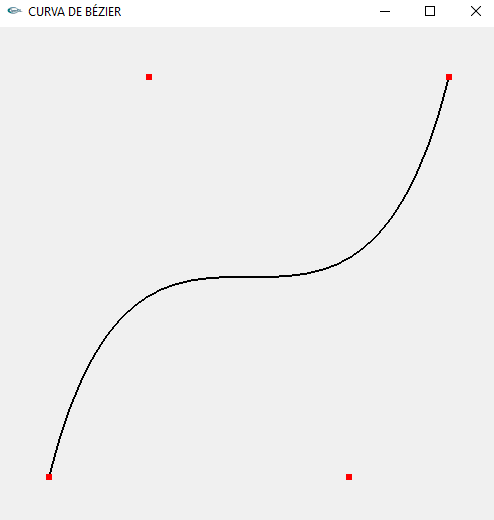
\includegraphics[width=0.5\linewidth]{../images/CURVA.PNG}
	\caption{Curva de Bézier.}
	\label{fig:propuesta}
\end{figure}
%%%%%%%%%%%%%%%%%%%%%%%%%%%%%%%%%%%%%%%%%%%%%%%%%%%%%%%%%%%%%%%%%%%%%%%%%%%%%%%%%%%%%%%%%%%%%%%%%%%%%%%%%%%%%%%%%%%%%%%%%%%%%%%%%%%%%%%%%%%%%%%%%%%%%%%%%%%%%%%%%%%%%%%%%%%%%%%%%%%%%%%%%%%%%%%%%%%%%%%%%%%%%%%%%%%%%%%%%%%%%%%%%%%%%%%%%%%%%%%%%%%%%%
\subsubsection{Código del ejemplo}

\lstset{language=C, breaklines=true, basicstyle=\footnotesize}
\begin{lstlisting}
#include <windows.h>
#include <GL/gl.h>
#include <GL/glu.h>
#include <stdlib.h>
#include <GL/glut.h>

GLfloat ctrlpoints[4][3] = {{ -4.0, -4.0, 0.0}, { -2.0, 4.0, 0.0},
                            {2.0, -4.0, 0.0}, {4.0, 4.0, 0.0}};

void init(void){
  glClearColor(0.0, 0.0, 0.0, 0.0);
  glShadeModel(GL_FLAT);
  glMap1f(GL_MAP1_VERTEX_3, 0.0, 1.0, 3, 4, &ctrlpoints[0][0]);
  glEnable(GL_MAP1_VERTEX_3);
}

void display(void){
      int i;
      glClear(GL_COLOR_BUFFER_BIT);
      glColor3f(1.0, 1.0, 1.0);

      glBegin(GL_LINE_STRIP);
        for (i = 0; i <= 30; i++)
            glEvalCoord1f((GLfloat) i/30.0);
      glEnd();

 /* El siguiente codigo muestra los puntos de control como puntos. */
      glPointSize(5.0);
      glColor3f(1.0, 1.0, 0.0);
      glBegin(GL_POINTS);
        for (i = 0; i < 4; i++)
          glVertex3fv(&ctrlpoints[i][0]);
      glEnd();

glFlush();
}

void reshape(int w, int h) {
      glViewport(0, 0, (GLsizei) w, (GLsizei) h);
      glMatrixMode(GL_PROJECTION);
      glLoadIdentity();

      if (w <= h)
        glOrtho(-5.0, 5.0, -5.0*(GLfloat)h/(GLfloat)w,
        5.0*(GLfloat)h/(GLfloat)w, -5.0, 5.0);
      else
      glOrtho(-5.0*(GLfloat)w/(GLfloat)h,
      5.0*(GLfloat)w/(GLfloat)h, -5.0, 5.0, -5.0, 5.0);
      glMatrixMode(GL_MODELVIEW);
      glLoadIdentity();
}

int main(int argc, char** argv) {
      glutInit(&argc, argv);
      glutInitDisplayMode (GLUT_SINGLE | GLUT_RGB);
      glutInitWindowSize (500, 500);
      glutInitWindowPosition (100, 100);
      glutCreateWindow (argv[0]);
      init ();
      glutDisplayFunc(display);
      glutReshapeFunc(reshape);
      glutMainLoop();
      return 0;
}
\end{lstlisting}

La curva cúbica de Bézier se describe mediante cuatro puntos de control, que aparecen en este ejemplo en la matriz \textbf{ctrlpoints[][]}. Esta matriz es uno de los argumentos de \textbf{glMap1f()}. Todos los argumentos de este comando son los siguientes:\\
\begin{itemize}
    \item \textbf{$GL\_MAP1\_VERTEX\_3$ :} Proporciona puntos de control tridimensionales y se producen vértices tridimensionales.
    \item \textbf{0.0: } Valor bajo del parámetro u
    \item \textbf{1.0: } Valor elevado del parámetro u
    \item \textbf{3: } El número de valores de punto flotante para avanzar en los datos entre un punto de control y el siguiente.
    \item \textbf{4: } El orden de la spline, que es el grado + 1: en este caso, el grado es 3 (ya que se trata de una curva cúbica ).
    \item \textbf{\&ctrlpoints[0][0]: } Puntero a los datos del primer punto de control
\end{itemize}
Nótese que el segundo y tercer argumento controlan la parametrización de la curva ya que la variable $u$ va de 0 a 1, la curva va de un extremo a otro. La llamada a \textbf{glEnable()} habilita el evaluador unidimensional para vértices tridimensionales. \\

La curva se dibuja en la rutina \textbf{display()} entre las llamadas \textbf{glBegin()} y \textbf{glEnd()}. Como el evaluador está habilitado, el comando \textbf{glEvalCoord1f()} es como emitir un comando \textbf{glVertex()} con las coordenadas de un vértice de la curva correspondiente al parámetro de entrada $u$.

%%%%%%%%%%%%%%%%%%%%%%%%%%%%%%%%%%%%%%%%%%%%%%%%%%%%%%%%%%%%%%%%%%%%%%%%%%%%%%%%%%%%%%%%%
\subsection{Definición y evaluación de un evaluador unidimensional}
El polinomio de Bernstein de grado n (u orden $n+1$ ) aproxima una función en un intervalo y viene dado por:

\begin{align*}
B_i^n\left(u\right)=\left(\begin{matrix}n\\i\\\end{matrix}\right)u^i\left(1-u\right)^{n-i}
\end{align*}
Si $Pi$ representa un conjunto de puntos de control (unidimensionales, bidimensionales, tridimensionales o incluso cuatridimensionales), entonces la ecuación:
\begin{align*}
C\left(u\right)=\sum_{i=0}^{n}{B_i^n\left(u\right)}P_i
\end{align*}
Donde los ${\displaystyle B_{i}^{n}(u)}$ son elementos de la distribución binomial respecto de la variable $u$ y los $P_{i}$ son valores de la función que queremos aproximar.\\

Representa una curva de Bézier cuando $u$ varía de 0 a 1. Para representar la misma curva, pero permitiendo que, $u$ varíe entre $u1$ y $u2$ en lugar de 0 y 1, evaluamos:
\begin{align*}
C\left(\frac{u-u_1}{u_2-u_1}\right)
\end{align*}
El comando \textbf{glMap1()} define un evaluador unidimensional que utiliza estas ecuaciones.\\

\begin{lstlisting}
    void glMap1(GLenum target,TYPE u1,TYPE u2,GLint stride,

                    GLint order,const TYPE *points);
\end{lstlisting}
El parámetro objetivo especifica lo que representan los puntos de control, como se muestra en la Tabla 1, y por lo tanto cuántos valores deben ser suministrados en puntos. Los puntos pueden representar vértices, datos de color RGBA, vectores normales o coordenadas de textura. Por ejemplo, con \textbf{$GL\_MAP1\_COLOR\_4$}, el evaluador genera datos de color a lo largo de una curva en el espacio de color de cuatro dimensiones (RGBA). También se utilizan los valores de los parámetros listados en la Tabla 1 para activar cada evaluador definido antes de invocarlo. Pase el valor apropiado a \textbf{glEnable()} o \textbf{glDisable()} para activar o desactivar el evaluador.\\

Los dos segundos parámetros de \textbf{glMap1*()}, $u1$ y $u2$, indican el rango de la variable $u$. La variable stride es el número de valores de precisión simple o doble (según el caso) en cada bloque de almacenamiento. Por lo tanto, es un valor de desplazamiento entre el comienzo de un punto de control y el comienzo del siguiente. \\

El orden es el grado más uno, y debe coincidir con el número de puntos de control. Los puntos apuntan a la primera coordenada del primer punto de control. Utilizando la estructura de datos de ejemplo para \textbf{glMap1*()}, utilice lo siguiente para los puntos:
\begin{align*}
(GLfloat \ *) (\&ctrlpoints[0].x)
\end{align*}

\begin{table}[h]
\begin{center}
\caption{Tipos de puntos de control para \textbf{glMap1*()}.}
	\arrayrulecolor{grayblack}
	%\rowcolors{1}{white}{gray}
	{\color{grayblack}
\begin{tabular}{ p{6.5cm} cc }
\toprule
\textbf{Parámetro } & \textbf{Significado} \\
\midrule
GL\_MAP1\_VERTEX\_3 & coordenadas de los vértices x, y, z.\\

GL\_MAP1\_VERTEX\_4 & coordenadas de los vértices x, y, z, w. \\
GL\_MAP1\_INDEX & índice de color. \\

GL\_MAP1\_COLOR\_4 & R, G, B, A. \\

GL\_MAP1\_NORMAL & coordenadas normales. \\

GL\_MAP1\_TEXTURE\_COORD\_1 & s coordenadas de textura. \\

GL\_MAP1\_TEXTURE\_COORD\_2 & s, t coordenadas de textura. \\

GL\_MAP1\_TEXTURE\_COORD\_3  & s, t, r coordenadas de textura \\

GL\_MAP1\_TEXTURE\_COORD\_4  & s, t, r, q coordenadas de textura. \\
\bottomrule
\end{tabular}}
\label{tab:coeficientes}
\end{center}
\end{table}

Se puede evaluar más de un evaluador a la vez. Se tiene un evaluador GL\_MAP1\_VERTEX\_3 y un evaluador GL\_MAP1\_COLOR\_4 definidos y habilitados, entonces las llamadas a \textbf{glEvalCoord1()} generan tanto una posición como un color. Sólo uno de los evaluadores de vértices puede estar habilitado a la vez, aunque se hayan definido ambos. Del mismo modo, sólo uno de los evaluadores de textura puede estar activo. Sin embargo, aparte de esto, los evaluadores pueden utilizarse para generar cualquier combinación de datos de vértices, vectores normales, colores y coordenadas de textura. Si se define y activa más de un evaluador del mismo tipo, se utiliza el de mayor dimensión. Utilizamos \textbf{glEvalCoord1*()} para evaluar un mapa unidimensional definido y habilitado.

\begin{lstlisting}
      void glEvalCoord1{fd}(TYPE u);
      void glEvalCoord1{fd} v (TYPE *u);
\end{lstlisting}
Provoca la evaluación de los mapas unidimensionales habilitados. El argumento $u$ es el valor (o un puntero al valor, en la versión vectorial del comando) de la coordenada del dominio. \\

%%%%%%%%%%%%%%%%%%%%%%%%%%%%%%%%%%%%%%%%%%%%%%%%%%%%%%%%%%%%%%%%%%%%%%%%%%%%%%%%%%%%%%%%%%%%%%%%
\subsection{Definición de valores de coordenadas uniformes en una dimensión}

Se utiliza \textbf{glEvalCoord1()} con cualquier valor para $u$, pero el uso más común es con valores espaciados uniformemente, como se muestra en el Ejemplo 1. Para obtener valores uniformemente espaciados, definimos una unidimensional usando \textbf{glMapGrid1*()} y luego aplíquelo usando \textbf{glEvalMesh1()}.

\begin{lstlisting}
    void glMapGrid1{fd} (GLint n, TYPE u1, TYPE u2);
\end{lstlisting}
Define una cuadrícula que va de $u1$ a $u2$ en $n$ pasos, que están espaciados uniformemente.
\begin{lstlisting}
    void glEvalMesh1(GLenum mode, GLint p1, GLint p2);
\end{lstlisting}

Aplicamos la cuadrícula de mapa definida actualmente a todos los evaluadores habilitados. El modo puede ser \textbf{GL\_POINT o GL\_LINE}, dependiendo de si desea dibujar puntos o una línea conectada a lo largo de la curva. La llamada tiene exactamente el mismo efecto que emitir una \textbf{glEvalCoord1()} para cada uno de los pasos, incluyendo $p1$ y $p2$, donde $0\le\ p1,\ p2\le\ n$. Es equivalente a lo siguiente: \\

\begin{lstlisting}
    glBegin(GL_POINTS); /* OR glBegin(GL_LINE_STRIP); */
          for (i = p1; i <= p2; i++)
              glEvalCoord1(u1 + i*(u2-u1)/n);
    glEnd();
\end{lstlisting}

Excepto que si $i = 0$ o $i = n$, entonces se llama a \textbf{glEvalCoord1()} con exactamente $u1$ o $u2$ como parámetro.

\newpage
% \bibliographystyle{plain} % We choose the "plain" reference style
% \bibliography{bibliography/biblio} % Entries are in the refs.bib file

\begin{thebibliography}{9}
    \bibitem{neider1993opengl}
    Neider, Jackie and Davis, Tom and Woo, Mason (1993) \emph{OpenGL programming guide}, Addison-Wesley Reading, MA
\end{thebibliography}

	% Bibliografia
	\newpage

	%\printbibliography[heading=bibintoc]
    
\end{document}